%%This is a very basic article template.
%%There is just one section and two subsections.
\documentclass{VLKlauck}
\usepackage{graphicx}
\usepackage{array}
\author[]{Christian Holl (24296)}
\institute[HTW Aaalen - Elektronik und Informatik]
{
	Studiengang Computer Controlled Systems\\
	Hochschule Aalen - Technik und Wirtschaft
}

\graphicspath{{./img/}}

\title[]{Online Symbolerkennung durch Datenfusion einer 3D und einer Farbkamera für einen autonomen Roboter}

\newcolumntype{S}{>{\centering\arraybackslash} m{.4\linewidth} }
	

\date[]{\today}  

\usepackage[right]{eurosym}
    
\begin{document}
\maketitle

  \section{Einleitung}
  \subsection{Aufgabenstellung}
	\begin{frame}{Aufgabenstellung}   
		\begin{itemize}
		  \item 3D-Kamera: Microsoft Kinect
		  \item Software: ROS (Robot Operating System \url{http://www.ros.org})
		  \item Finden von Oberflächen mit passenden Eigenschaften:
		 	 \begin{itemize}
		    	\item Ausrichtung (senkrecht zum Betrachter) 
		    	\item Größe 
		    	\item Ort
		    	\item Entfernung   
			\end{itemize}
		  \item Durchsuchen der Oberflächen nach bekannten Symbolen
		\end{itemize}
		Hintergrund: Schnelleres Auffinden von Schildern in Kamerabildern
	\end{frame} 
	\subsection{Funktionsweise Kinect} 
	\begin{frame}{Kinect: Übersicht}
		Tiefenkamera und Farbkamera in einem (Preis \textasciitilde \EUR{110})  
		
		\begin{tabular}{cc}
			Übersicht 								   & Bild IR-Sensor\\
			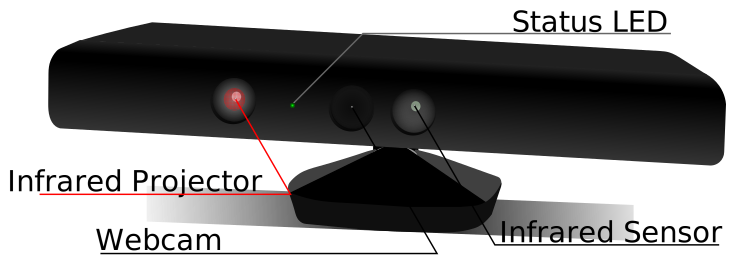
\includegraphics[scale=0.3]{Kinect.pdf}  & \includegraphics[scale=0.4]{ir_kinect.png}\\	
		\end{tabular}  
		
	\end{frame}
	

	\begin{frame}{Kinect Funktionsweise} 
		
		\begin{tabular}{SS}
			Laserscanner							   & Kinect\\
			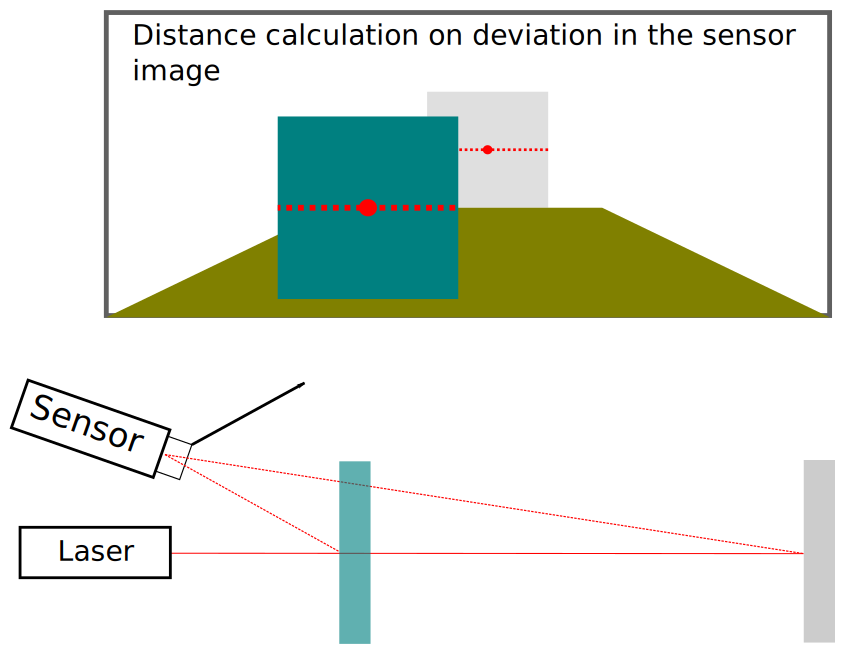
\includegraphics[scale=0.18]{laserScannerPrinciple.pdf}  & 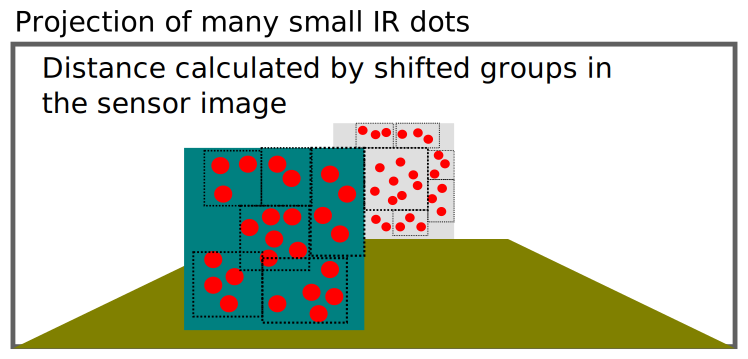
\includegraphics[scale=0.18]{kinect_principle.pdf}\\	
		\end{tabular} 
	\end{frame}
	
	\subsection{ROS(Publisher Subscriber Pattern)}
	\begin{frame}{ROS(Publisher Subscriber Pattern)}
		\centering
			Beispiel Realität\\					   
			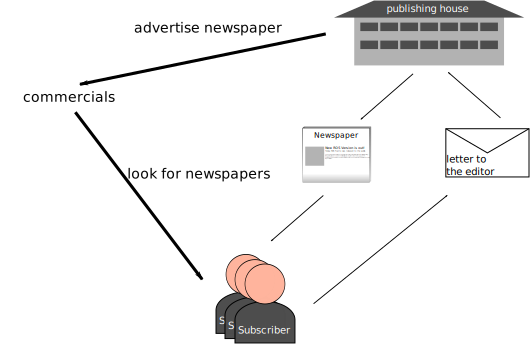
\includegraphics[scale=0.5]{PS_Newspaper.pdf}
	\end{frame}
	
 	\begin{frame}{ROS(Publisher Subscriber Pattern)}
		\centering
		Beispiel ROS\\			   
		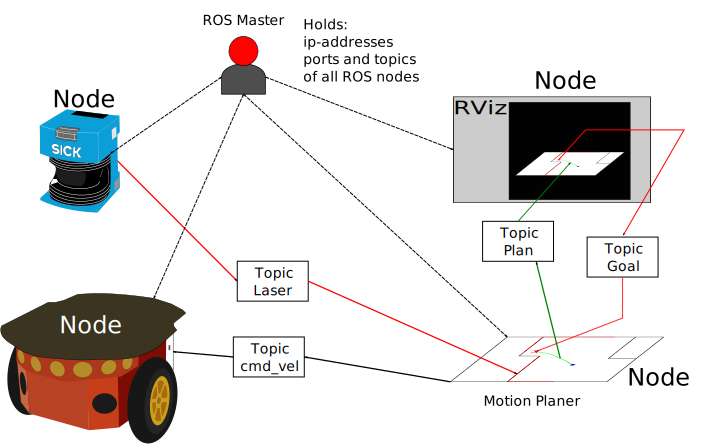
\includegraphics[scale=0.5]{PS_ROS.pdf}
	\end{frame}
	
	\subsection{Mechanik}
	\begin{frame}{Mechanik}
		\begin{tabular}{cc}
			Schilder 								   & Änderungen am Roboter\\
			\includegraphics[scale=0.07]{signs.jpg}  & \includegraphics[scale=0.1]{laptop_stand_side.png}\\	
		\end{tabular}
	\end{frame} 
	  
	
	\section{Kinect Analyse} 
	\subsection{Tools}
	
	\begin{frame}{DepthImageAnalyzer (Qt Node)}
		\includegraphics[scale=0.2]{DepthImageAnalyzer.jpg}
	\end{frame}
	
	\begin{frame}{Rviz}
		\includegraphics[scale=0.4]{RVizPointCloud.png}
	\end{frame} 
	
	\begin{frame}{Node mit PointCloud}
		\includegraphics[scale=0.35]{disturbance_filter_calibrator1.png}	
	\end{frame}
	
	
	\subsection{Probleme mit Oberflächen}
		
	\begin{frame}{\insertsubsection: Zu Nah}	
		\includegraphics[scale=0.4]{ToClose.png}
	\end{frame}
			
	\begin{frame}{\insertsubsection: Sonneneinstrahlung}	
		\includegraphics[scale=1.2]{Sun.png}
	\end{frame}
			
	\begin{frame}{\insertsubsection: Spiegelnde Flächen}	
		\includegraphics[scale=0.8]{Mirror.png}
	\end{frame}
	
	\begin{frame}{\insertsubsection: Transparente Materialien}	
		\includegraphics[scale=1]{glas.png} 	
	\end{frame}
	
	\subsection{Ergebnisse}
	
	\begin{frame}{\insertsubsection: Abweichungen über die Distanz}	
	\includegraphics[scale=0.6]{LaserDistanceKinectDistance.png}
    \end{frame}
    
    \begin{frame}{\insertsubsection: Vorhandene Werte bis 4838mm}
	\moveleft9mm\hbox{\includegraphics[scale=0.073]{availdepths0.png}}
	\end{frame}
	
	\begin{frame}{\insertsubsection: Vorhandene Werte bis 9757mm}	
	\moveleft9mm\hbox{\includegraphics[scale=0.073]{availdepths1.png}}
	\end{frame}
	
	\begin{frame}{\insertsubsection: Abstand zwischen den Werten nach Tiefe}	
	\includegraphics[width=\textwidth]{DifferenceForegoing.png}
	\end{frame}
	
	
	\subsection{Bildrauschen und Kameraverhalten}
	\begin{frame}{\insertsubsection}	
	    \includegraphics[scale=0.5]{noise.png}
	\end{frame}
	
	\begin{frame}{\insertsubsection}	
		\includegraphics[scale=0.3]{verticalFractals.png}
	\end{frame}	
	
	
	%%%%%%%%%%%%%%%%%%%%%%%%%%%%%%%%%%%%%%%%%%%%%%%%%%
	%SOFTWARE										 %
	%%%%%%%%%%%%%%%%%%%%%%%%%%%%%%%%%%%%%%%%%%%%%%%%%%
	\section{Software}  
	\subsection{Bildbeschaffung}
	\begin{frame}{\insertsubsection}
		\begin{itemize}
		  \item OpenNI-Node (für Kinect Kamera):
		  \begin{itemize}	
		    \item RGB-Bild
		    \item Depth-Bild
		    \item camera\_info (Enthält: Kameraparameter, Kalibrierung etc.)
		  \end{itemize}
		  \item Eigene Node (Code von XYZRGB Nodelet)
		\end{itemize}
	\end{frame}
	
	
	
	
	\subsection{Weichzeichnen}
	\begin{frame}{\insertsubsection: OpenCV Funktionen und Rücksetzen von Pixeln (1.Methode)}
	\begin{itemize}
     \item Boxed Filter (Blendengröße 7*3)
     \item Median Filter (3*3)
     \item Rücksetzen der Pixel, die zu weit von Originalwert entfernt sind, mit folgender Funktion:\\
   			$$
      			\left(\left|{P_b(x,y)-P(x,y)}\right|>{\frac{P(x,y)^2}{480000}}\right)\implies P_b(x,y)=P(x,y)
			$$
	 \item Erneuter Median Filter (3*3)
    \end{itemize}
	\end{frame}
	
	\begin{frame}{\insertsubsection: OpenCV Funktionen und Rücksetzen von Pixeln (1.Methode)}
			\includegraphics[width=\textwidth]{myFilter1.png}
	\end{frame}
	 
	 	
	\begin{frame}{\insertsubsection: Erstellen einer Nachbarschaftskarte und Kreuzweichzeichner (2.Methode)}

	Umwandeln des Tiefenbildes in ein Schrittbild (Step-Map) mittels Look-Up-Table:\\[0.5cm]
	{
	\tiny
		  \begin{tabular}{lccccccccccc}
			Kinect Depth& 0 & 317 & 318 & 319 &  ...  & 8550 & 8767 & 8995 & 9235 & 9489 & 9757\\
			Step Number & 0 &   1 &   2 &   3 &  ...  &  819 &  820 &  821 &  822 & 823  & 824\\
		  \end{tabular}
	}\\[0.5cm]

			Beispiel:\\
			\begin{tabular}{ccc} 
			0 & 320 & 321\\
			8146 & 8550 & 9489\\
			\end{tabular}\\[0.5cm]

			Wird zu:\\
			\begin{tabular}{ccc}
			0 & 4 & 5\\
			817 & 819 & 823\\
			\end{tabular}
	\end{frame}
	 
	\begin{frame}{\insertsubsection: Erstellen einer Nachbarschaftskarte und Kreuzweichzeichner (2.Methode)}
	 	Erstellen des Nachbarschaftsbilds (neighborhood-map):\\[0.5cm]
	 	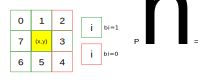
\includegraphics[width=\textwidth]{neighborhoodmap.pdf}\\
	 	{\tiny
	 	$$
	 	 b_i = \left\{ 
	 	\begin{array}{ll}
	         1 & \left|S(x_i,y_i)-S(x,y)\right|<4  \wedge   S(x_i,y_i) \neq 0 \wedge 0<=x_i<u  \wedge 0<=y_i<v\\
	         0 & \mbox{otherwise} 
	 	\end{array}
		\right.   
	 	$$
	 	}
	\end{frame}
	  
	\begin{frame}{\insertsubsection: Erstellen einer Nachbarschaftskarte und Kreuzweichzeichner (2.Methode)}
	 	Weichzeichnen mittels Kreuzweichzeichner:\\[0.5cm]
	 	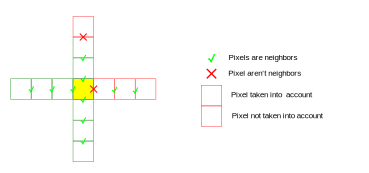
\includegraphics[width=\textwidth]{crossBlur.pdf}
	\end{frame}
	   
	   
	\begin{frame}{\insertsubsection: Erstellen einer Nachbarschaftskarte und Kreuzweichzeichner (2.Methode)}
	   Ergebnis:
	   \includegraphics[width=\textwidth]{crossBlurResult.png}
	\end{frame}
	   
	\subsection{Koordinatenberechnung und Filterung}
	\begin{frame}{Realkoordinaten X und Y}
	$$X(x,y)=\frac{(x-center_x) \cdot D(x,y)}{f_x}$$
	$$Y(x,y)=\frac{(y-center_y) \cdot D(x,y)}{f_y}$$
	$D(x,y):$ Z-Wert von Pixel (x,y)\\
	$center_x :$ Mitte des Bildes in x-Richtung (Pixel)\\
	$center_y :$ Mitte des Bildes in y-Richtung (Pixel)\\	
	$f_x:$ Fokale Distanz in x-Richtung\\
	$f_y:$ Fokale Distanz in y-Richtung
	
	(*Berechnungsformel aus XYZRGB Nodelet entnommen)
	
	\end{frame}
	   
	\begin{frame}{3D Range Filter}
	 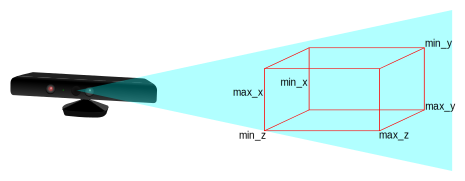
\includegraphics[width=\textwidth]{XYZFilter.pdf}
	 {\tiny
	 \begin{equation}
 	 \begin{split}
 	   	(X < Xmin \vee X > Xmax \vee Y > Ymax \vee Y < Ymin \vee D(x,y) < Zmin \vee D(x,y) > Zmax)\\
 	   	\implies D_{out}(x,y) = 0    	   
 	 \end{split}
 	 \nonumber
	\end{equation}
	} 	 
	\end{frame}
	
	
	\subsection{Normale und Winkel}
	\begin{frame}{Berechnung der Normale}
	
	{\tiny
			\begin{equation}
		 		\vec{N} =        \left( \begin{array}{c} x_u                           \\                           y_u \\ z_u                           \end{array} \right) 
		           \times \left( \begin{array}{c} x_v                           \\                           y_v \\ z_v                           \end{array} \right) 
		         =        \left( \begin{array}{c} y_u \cdot z_v - z_u \cdot y_v \\ z_u \cdot x_v - z_v \cdot x_u \\ x_u \cdot y_v - y_u \cdot x_v \end{array}\right)
				\nonumber
			\end{equation}
			\begin{gather}
		 \vec{N}_{tr}(x,y)=    \vec{V}_t(x,y) \times \vec{V}_r(x,y) =
		                  \left( \begin{array}{c}   X(x,y-1) -  X(x,y)  \\ Y(x,y-1) -  Y(x,y) \\ D(x,y-1) -  D(x,y)\end{array} \right) 
		           \times \left( \begin{array}{c}   X(x+1,y) -  X(x,y)  \\ Y(x+1,y) -  Y(x,y) \\ D(x+1,y) -  D(x,y)\end{array} \right)\nonumber\\
		 \vec{N}_{bl}(x,y)=    \vec{V}_b(x,y) \times \vec{V}_l(x,y) =
		                  \left( \begin{array}{c}   X(x,y+1) -  X(x,y)  \\ Y(x,y+1) -  Y(x,y) \\ D(x,y+1) -  D(x,y)\end{array} \right) 
		           \times \left( \begin{array}{c}   X(x-1,y) -  X(x,y)  \\ Y(x-1,y) -  Y(x,y) \\ D(x-1,y) -  D(x,y)\end{array} \right)\nonumber
		\end{gather}
	}
	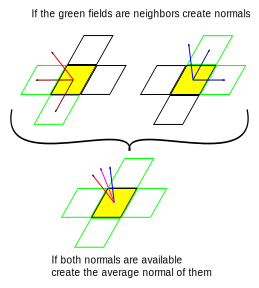
\includegraphics[scale=0.5]{normals.pdf}
	\end{frame}
	   
	\begin{frame}{Winkel zu x,y und z-Achse}
		  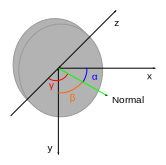
\includegraphics[scale=0.9]{Angles.pdf}
		\begin{align}
		 \alpha = \arccos \frac{N_x}{\left|\vec{N}\right|}  
		\nonumber\\
		 \gamma = \arccos \frac{N_z}{\left|\vec{N}\right|}  
		\nonumber\\
		 \beta  = \arccos \frac{N_y}{\left|\vec{N}\right|}  
		\nonumber
		\end{align} 
	\end{frame}
	
	
	\begin{frame}{Winkelweichzeichnen / Filtern nach Winkel}
		Weichzeichnen des Winkelbildes mit dem vorherigen Kreuzweichzeichner\\
		\includegraphics[width=\textwidth]{AnglesMapBlured.png}\\
		Filtern nach Winkel -> Schwarz/Weiß Bild
	\end{frame}
	
	
	
	\subsection{Flächensegmentierung und Bildentzerrung}
	\begin{frame}{Flächensegmentierung}
		ID-Vergabe und Erstellen von ID-Relationen
		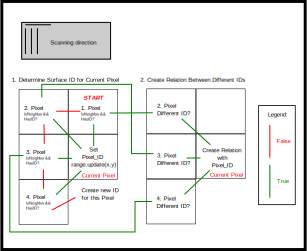
\includegraphics[scale=0.8]{SurfaceSegmentation.pdf}
	\end{frame}
	
	\begin{frame}{Flächensegmentierung und Filterung}
		ID-Zusammenführung
		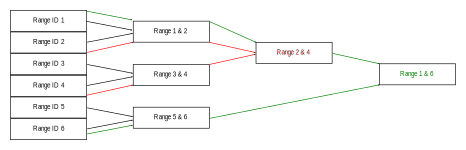
\includegraphics[scale=0.8]{merging.pdf}\\
		\includegraphics[scale=0.8]{AnglesOkSegment.png}
		
		Anschließend Filterung nach Flächengröße (Min/Max)
	\end{frame}

	\begin{frame}{Perspektivische Entzerrung}
		Entzerrung mittels OpenCV warpPerspektive.\\
		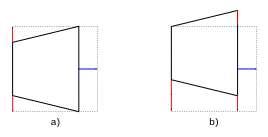
\includegraphics[scale=0.8]{PerspectiveTransform.pdf}\\ 
		\includegraphics[scale=1]{warpPerspective.png}
	\end{frame}
	
	\subsection{Template Matching}
	\begin{frame}{\insertsubsection: 1.Methode}
		\begin{tabular}{cc}
			HSV-Filter auf Bild 								   & Resultat:\\
			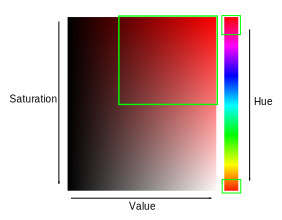
\includegraphics[scale=0.6]{HSV.pdf}  & \includegraphics[scale=0.7]{redFilterResult.png}\\	
		\end{tabular} 
		
		Anschließende Kreisfindung mit hughCircles und Kreisposition mit Template vergleichen
		
	\end{frame}
	\begin{frame}{\insertsubsection: Problem 1.Methode}
		  
\includegraphics[scale=0.4]{robotSignProblem.pdf}
	\end{frame}
	\begin{frame}{\insertsubsection: 2.Methode}
		{Analysieren der Template Proportionen}
		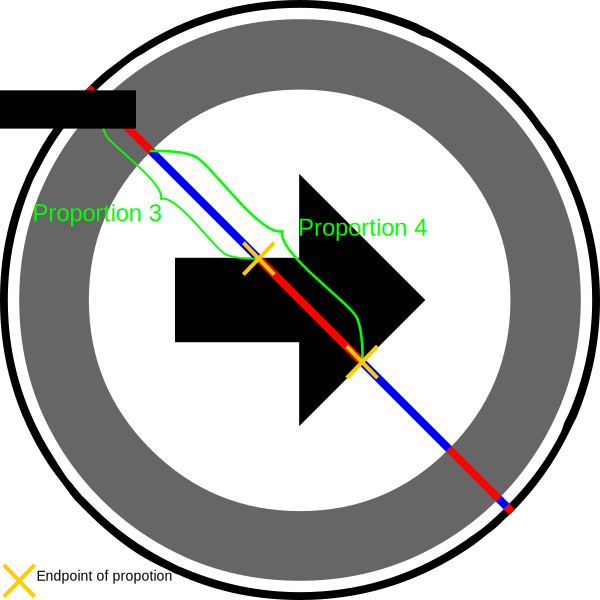
\includegraphics[scale=0.35]{proportionGather.pdf}
	\end{frame}	
	
	\begin{frame}{\insertsubsection: 2.Methode}
		{\small Suchen nach bekannten Proportionspaaren im entzerrten Kamerabild}
		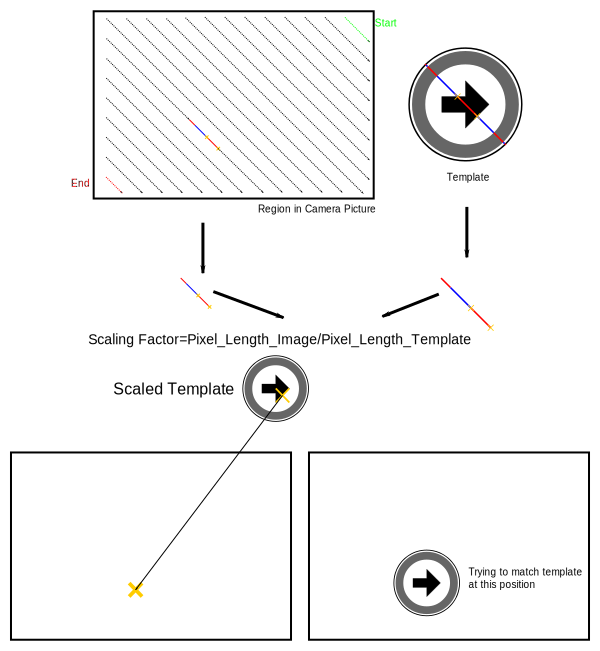
\includegraphics[scale=0.45]{FindingProportions.pdf}
	\end{frame}
	
	
	\begin{frame}{\insertsubsection: 2.Methode}
	{Resultat}
	\includegraphics[width=\textwidth]{three.png}
	\end{frame}

	\section{Zusammenfassung}
   \begin{frame}
     \frametitle{Zusammenfassung}
     \tableofcontents[sectionstyle=show/hide, subsectionstyle=hide/hide/hide]
   \end{frame}

	\begin{frame}{\insertsection}
		\begin{itemize}
	  		\item Nachbarschaftskarte ermöglicht es Performance in allen Schritten 
	  		       einzusparen
			\item nachbarschaftsorientierter Kreuzweichzeichner 
	  			   führt zu guten Ergebnissen ohne spürbare Verzögerung
			\item Alle Prozessschritte bis einschließlich Winkelweichzeichnung
		           einfach parallelisierbar (z.B. durch NVIDIA CUDA)
		    \item \textbf{Der Flächenausschluss über Größen führt im Gegensatz
		           zum template Matching ohne Flächenausschluss zu einer deutlich
		           höheren Bildrate, das Bild wird in den meisten Fällen einigermaßen
		           flüssig dargestellt}
		\end{itemize}
	\end{frame}
	\begin{frame}{\insertsection}
		Probleme:
		\begin{itemize}
		  \item Ähnliche Symbole erfordern eine niedrige Toleranz beim template Matching\\
		         \textbf{Folge:} nicht in jedem Frame wird ein Schild gefunden
		  \item Nachbarschaftskarte funktioniert aktuell nur bei harten Kanten
				 (Lösung: Einbeziehung von Gradienten)
		\end{itemize}
	\end{frame}   
	\begin{frame}{Vielen Dank für Ihre Aufmerksamkeit}
	    \begin{itemize}
	      \item Dokumentation und Quellcode(comming sooner or later):\\
	      {\small\url{http://radiationlaboratories.blogspot.de/2012/07/online-symbol-recognition-through-data.html}}\\
	       (Shortlink: \url{http://tinyurl.com/OSR-3D-RGB})\\ \includegraphics[scale=1]{qrLink.png}
	    \end{itemize}
	\end{frame} 



\end{document}
  